\documentclass{standalone}
\usepackage{tikz}
\usetikzlibrary{patterns, positioning}

\begin{document}
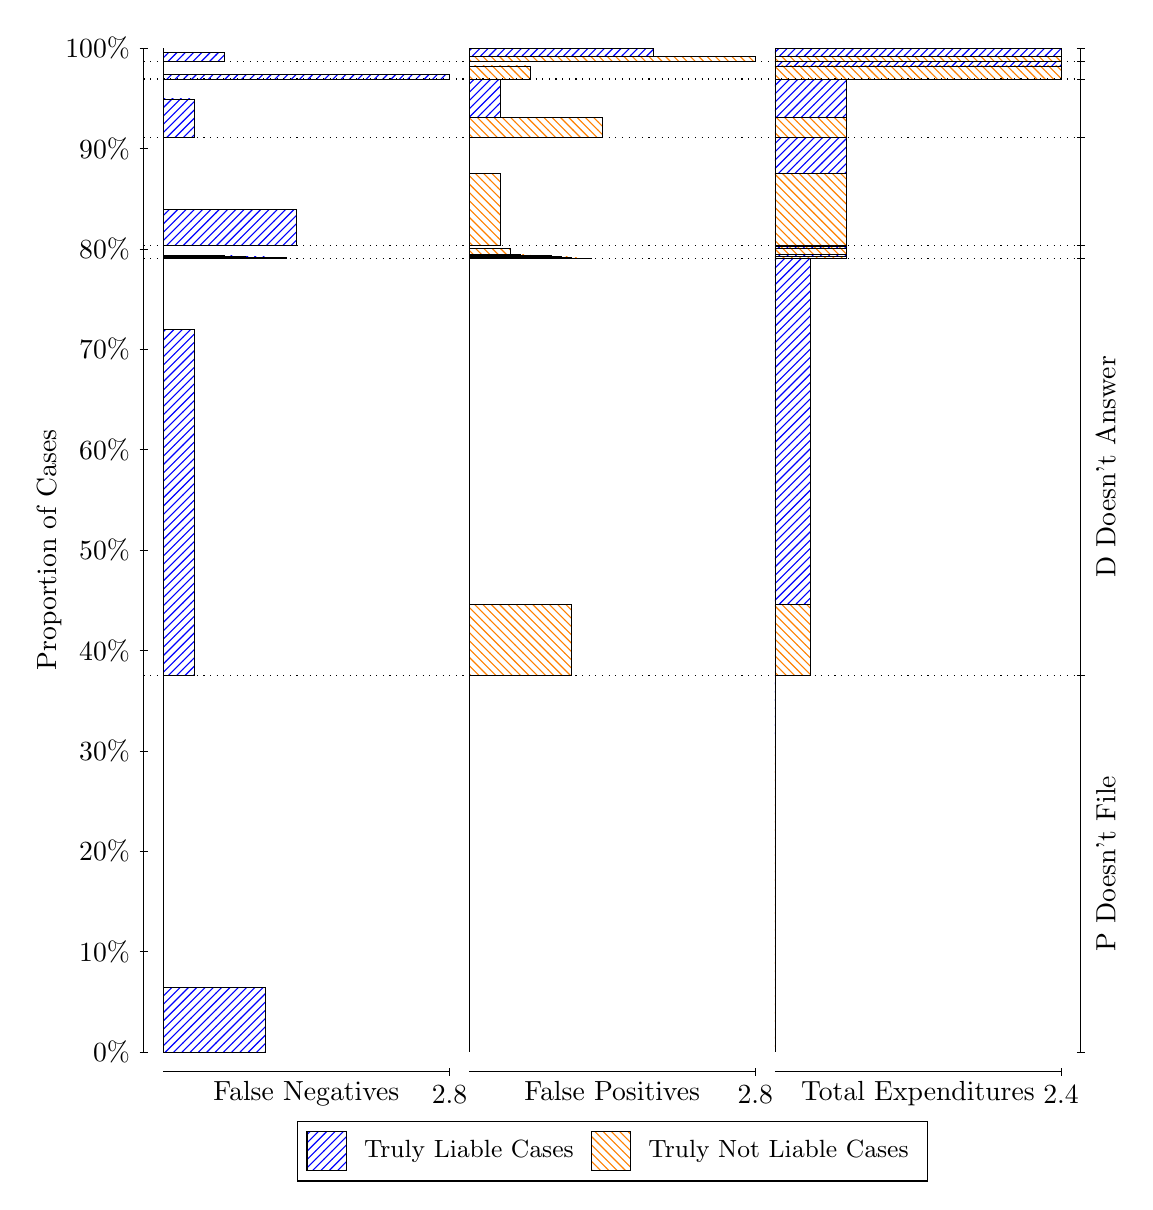
\begin{tikzpicture}
\draw[black, very thin] (1.5,1.75) -- (1.5,14.5);
\node[rotate=90, anchor=center] at (0.3, 8.125) {Proportion of Cases};
\draw[black, very thin] (1.45,1.75) -- (1.55,1.75);
\node[anchor=east] at (1.45, 1.75) {0\%};
\draw[black, very thin] (1.45,3.025) -- (1.55,3.025);
\node[anchor=east] at (1.45, 3.025) {10\%};
\draw[black, very thin] (1.45,4.3) -- (1.55,4.3);
\node[anchor=east] at (1.45, 4.3) {20\%};
\draw[black, very thin] (1.45,5.575) -- (1.55,5.575);
\node[anchor=east] at (1.45, 5.575) {30\%};
\draw[black, very thin] (1.45,6.85) -- (1.55,6.85);
\node[anchor=east] at (1.45, 6.85) {40\%};
\draw[black, very thin] (1.45,8.125) -- (1.55,8.125);
\node[anchor=east] at (1.45, 8.125) {50\%};
\draw[black, very thin] (1.45,9.4) -- (1.55,9.4);
\node[anchor=east] at (1.45, 9.4) {60\%};
\draw[black, very thin] (1.45,10.675) -- (1.55,10.675);
\node[anchor=east] at (1.45, 10.675) {70\%};
\draw[black, very thin] (1.45,11.95) -- (1.55,11.95);
\node[anchor=east] at (1.45, 11.95) {80\%};
\draw[black, very thin] (1.45,13.225) -- (1.55,13.225);
\node[anchor=east] at (1.45, 13.225) {90\%};
\draw[black, very thin] (1.45,14.5) -- (1.55,14.5);
\node[anchor=east] at (1.45, 14.5) {100\%};

\draw[black, very thin] (13.4,1.75) -- (13.4,14.5);
\draw[black, very thin] (13.35,1.75) -- (13.45,1.75);
\node[anchor=west] at (13.35, 1.75) {};
\draw[black, very thin] (13.35,6.5326) -- (13.45,6.5326);
\node[anchor=west] at (13.35, 6.5326) {};
\draw[black, very thin] (13.35,11.83) -- (13.45,11.83);
\node[anchor=west] at (13.35, 11.83) {};
\draw[black, very thin] (13.35,11.994) -- (13.45,11.994);
\node[anchor=west] at (13.35, 11.994) {};
\draw[black, very thin] (13.35,13.366) -- (13.45,13.366);
\node[anchor=west] at (13.35, 13.366) {};
\draw[black, very thin] (13.35,14.106) -- (13.45,14.106);
\node[anchor=west] at (13.35, 14.106) {};
\draw[black, very thin] (13.35,14.333) -- (13.45,14.333);
\node[anchor=west] at (13.35, 14.333) {};
\draw[black, very thin] (13.35,14.5) -- (13.45,14.5);
\node[anchor=west] at (13.35, 14.5) {};

\draw[black, very thin, pattern color=blue, pattern=north east lines] (1.75,1.75) rectangle (3.0476,2.5732);
\draw[black, very thin, pattern color=orange, pattern=north west lines] (1.75,2.5732) rectangle (1.75,6.5326);
\draw[black, very thin, pattern color=blue, pattern=north east lines] (1.75,6.5326) rectangle (2.1393,10.931);
\draw[black, very thin, pattern color=orange, pattern=north west lines] (1.75,10.931) rectangle (1.75,11.83);
\draw[black, very thin, pattern color=blue, pattern=north east lines] (1.75,11.83) rectangle (3.3071,11.843);
\draw[black, very thin, pattern color=blue, pattern=north east lines] (1.75,11.843) rectangle (3.1774,11.845);
\draw[black, very thin, pattern color=blue, pattern=north east lines] (1.75,11.845) rectangle (3.0476,11.847);
\draw[black, very thin, pattern color=blue, pattern=north east lines] (1.75,11.847) rectangle (2.9179,11.847);
\draw[black, very thin, pattern color=blue, pattern=north east lines] (1.75,11.847) rectangle (2.9179,11.848);
\draw[black, very thin, pattern color=blue, pattern=north east lines] (1.75,11.848) rectangle (2.7881,11.856);
\draw[black, very thin, pattern color=blue, pattern=north east lines] (1.75,11.856) rectangle (2.6583,11.859);
\draw[black, very thin, pattern color=blue, pattern=north east lines] (1.75,11.859) rectangle (2.5286,11.865);
\draw[black, very thin, pattern color=blue, pattern=north east lines] (1.75,11.865) rectangle (2.3988,11.868);
\draw[black, very thin, pattern color=blue, pattern=north east lines] (1.75,11.868) rectangle (2.269,11.871);
\draw[black, very thin, pattern color=orange, pattern=north west lines] (1.75,11.871) rectangle (1.75,11.994);
\draw[black, very thin, pattern color=blue, pattern=north east lines] (1.75,11.994) rectangle (3.4369,12.452);
\draw[black, very thin, pattern color=orange, pattern=north west lines] (1.75,12.452) rectangle (1.75,13.366);
\draw[black, very thin, pattern color=blue, pattern=north east lines] (1.75,13.366) rectangle (2.1393,13.853);
\draw[black, very thin, pattern color=orange, pattern=north west lines] (1.75,13.853) rectangle (1.75,14.106);
\draw[black, very thin, pattern color=blue, pattern=north east lines] (1.75,14.106) rectangle (5.3833,14.166);
\draw[black, very thin, pattern color=orange, pattern=north west lines] (1.75,14.166) rectangle (1.75,14.333);
\draw[black, very thin, pattern color=blue, pattern=north east lines] (1.75,14.333) rectangle (2.5286,14.44);
\draw[black, very thin, pattern color=orange, pattern=north west lines] (1.75,14.44) rectangle (1.75,14.5);
\draw[black, very thin, pattern color=orange, pattern=north west lines] (5.6333,1.75) rectangle (5.6333,5.7094);
\draw[black, very thin, pattern color=blue, pattern=north east lines] (5.6333,5.7094) rectangle (5.6333,6.5326);
\draw[black, very thin, pattern color=orange, pattern=north west lines] (5.6333,6.5326) rectangle (6.931,7.431);
\draw[black, very thin, pattern color=blue, pattern=north east lines] (5.6333,7.431) rectangle (5.6333,11.83);
\draw[black, very thin, pattern color=orange, pattern=north west lines] (5.6333,11.83) rectangle (7.1905,11.832);
\draw[black, very thin, pattern color=orange, pattern=north west lines] (5.6333,11.832) rectangle (7.0607,11.836);
\draw[black, very thin, pattern color=orange, pattern=north west lines] (5.6333,11.836) rectangle (6.931,11.848);
\draw[black, very thin, pattern color=orange, pattern=north west lines] (5.6333,11.848) rectangle (6.8012,11.855);
\draw[black, very thin, pattern color=orange, pattern=north west lines] (5.6333,11.855) rectangle (6.6714,11.866);
\draw[black, very thin, pattern color=orange, pattern=north west lines] (5.6333,11.866) rectangle (6.5417,11.868);
\draw[black, very thin, pattern color=orange, pattern=north west lines] (5.6333,11.868) rectangle (6.4119,11.873);
\draw[black, very thin, pattern color=orange, pattern=north west lines] (5.6333,11.873) rectangle (6.2821,11.878);
\draw[black, very thin, pattern color=orange, pattern=north west lines] (5.6333,11.878) rectangle (6.1524,11.953);
\draw[black, very thin, pattern color=blue, pattern=north east lines] (5.6333,11.953) rectangle (5.8929,11.955);
\draw[black, very thin, pattern color=blue, pattern=north east lines] (5.6333,11.955) rectangle (5.7631,11.958);
\draw[black, very thin, pattern color=blue, pattern=north east lines] (5.6333,11.958) rectangle (5.6333,11.994);
\draw[black, very thin, pattern color=orange, pattern=north west lines] (5.6333,11.994) rectangle (6.0226,12.909);
\draw[black, very thin, pattern color=blue, pattern=north east lines] (5.6333,12.909) rectangle (5.6333,13.366);
\draw[black, very thin, pattern color=orange, pattern=north west lines] (5.6333,13.366) rectangle (7.3202,13.619);
\draw[black, very thin, pattern color=blue, pattern=north east lines] (5.6333,13.619) rectangle (6.0226,14.106);
\draw[black, very thin, pattern color=orange, pattern=north west lines] (5.6333,14.106) rectangle (6.4119,14.272);
\draw[black, very thin, pattern color=blue, pattern=north east lines] (5.6333,14.272) rectangle (5.6333,14.333);
\draw[black, very thin, pattern color=orange, pattern=north west lines] (5.6333,14.333) rectangle (9.2667,14.393);
\draw[black, very thin, pattern color=blue, pattern=north east lines] (5.6333,14.393) rectangle (7.969,14.5);
\draw[black, very thin, pattern color=orange, pattern=north west lines] (9.5167,1.75) rectangle (9.5167,5.7094);
\draw[black, very thin, pattern color=blue, pattern=north east lines] (9.5167,5.7094) rectangle (9.5167,6.5326);
\draw[black, very thin, pattern color=orange, pattern=north west lines] (9.5167,6.5326) rectangle (9.9708,7.431);
\draw[black, very thin, pattern color=blue, pattern=north east lines] (9.5167,7.431) rectangle (9.9708,11.83);
\draw[black, very thin, pattern color=orange, pattern=north west lines] (9.5167,11.83) rectangle (10.425,11.858);
\draw[black, very thin, pattern color=blue, pattern=north east lines] (9.5167,11.858) rectangle (10.425,11.875);
\draw[black, very thin, pattern color=orange, pattern=north west lines] (9.5167,11.875) rectangle (10.425,11.961);
\draw[black, very thin, pattern color=blue, pattern=north east lines] (9.5167,11.961) rectangle (10.425,11.979);
\draw[black, very thin, pattern color=orange, pattern=north west lines] (9.5167,11.979) rectangle (10.425,11.988);
\draw[black, very thin, pattern color=blue, pattern=north east lines] (9.5167,11.988) rectangle (10.425,11.994);
\draw[black, very thin, pattern color=orange, pattern=north west lines] (9.5167,11.994) rectangle (10.425,12.909);
\draw[black, very thin, pattern color=blue, pattern=north east lines] (9.5167,12.909) rectangle (10.425,13.366);
\draw[black, very thin, pattern color=orange, pattern=north west lines] (9.5167,13.366) rectangle (10.425,13.619);
\draw[black, very thin, pattern color=blue, pattern=north east lines] (9.5167,13.619) rectangle (10.425,14.106);
\draw[black, very thin, pattern color=orange, pattern=north west lines] (9.5167,14.106) rectangle (13.15,14.272);
\draw[black, very thin, pattern color=blue, pattern=north east lines] (9.5167,14.272) rectangle (13.15,14.333);
\draw[black, very thin, pattern color=orange, pattern=north west lines] (9.5167,14.333) rectangle (13.15,14.393);
\draw[black, very thin, pattern color=blue, pattern=north east lines] (9.5167,14.393) rectangle (13.15,14.5);
\draw[black, dotted] (1.5,6.5326) -- (13.4,6.5326);
\draw[black, dotted] (1.5,11.83) -- (13.4,11.83);
\draw[black, dotted] (1.5,11.994) -- (13.4,11.994);
\draw[black, dotted] (1.5,13.366) -- (13.4,13.366);
\draw[black, dotted] (1.5,14.106) -- (13.4,14.106);
\draw[black, dotted] (1.5,14.333) -- (13.4,14.333);
\draw[black, very thin] (1.75,1.5) -- (5.3833,1.5);
\node[anchor=north] at (3.5667, 1.5) {False Negatives};
\draw[black, very thin] (5.3833,1.45) -- (5.3833,1.55);
\node[anchor=north] at (5.3833, 1.45) {2.8};

\draw[black, very thin] (5.6333,1.5) -- (9.2667,1.5);
\node[anchor=north] at (7.45, 1.5) {False Positives};
\draw[black, very thin] (9.2667,1.45) -- (9.2667,1.55);
\node[anchor=north] at (9.2667, 1.45) {2.8};

\draw[black, very thin] (9.5167,1.5) -- (13.15,1.5);
\node[anchor=north] at (11.333, 1.5) {Total Expenditures};
\draw[black, very thin] (13.15,1.45) -- (13.15,1.55);
\node[anchor=north] at (13.15, 1.45) {2.4};

\node[black, centered, rotate=90] at (13.72, 4.1413) {P Doesn't File};
\node[black, centered, rotate=90] at (13.72, 9.1812) {D Doesn't Answer};






\draw (7.449999999999999,1.5) node[draw=none] (baseCoordinate) {};
\begin{scope}[align=center]
        \matrix[scale=0.5, draw=black, below=0.5cm of baseCoordinate, nodes={draw}, column sep=0.1cm]{
            \node[rectangle, draw, minimum width=0.5cm, minimum height=0.5cm, pattern=north east lines, pattern color=blue] {}; &
            \node[draw=none, font=\small] (B) {Truly Liable Cases}; &
            \node[rectangle, draw, minimum width=0.5cm, minimum height=0.5cm, pattern=north west lines, pattern color=orange] {}; &
            \node[draw=none, font=\small] (B) {Truly Not Liable Cases}; \\
            };
\end{scope}

\end{tikzpicture}
\end{document}